\documentclass[12pt]{article}  % standard LaTeX, 12 point type

\usepackage{geometry}

\usepackage{amsmath}
\usepackage{amsfonts,latexsym}
\usepackage{amsthm}
\usepackage{amssymb}
\usepackage[utf8]{inputenc} % Кодировка
\usepackage[english,russian]{babel} % Многоязычность
\usepackage{algpseudocode}
\usepackage{algorithm}
\usepackage{algorithmicx}
\usepackage{verbatim}
\usepackage[toc,page]{appendix}

\usepackage{array}
\usepackage{multirow}
\usepackage{color}
\usepackage{listings}
\usepackage{caption}
\usepackage{graphicx}
\usepackage{ucs}

\newtheorem{theorem}{Theorem}[section]
\newtheorem{proposition}[theorem]{Proposition}
\newtheorem{lemma}[theorem]{Lemma}
\newtheorem{corollary}[theorem]{Corollary}
\newtheorem{conjecture}[theorem]{Conjecture}

\theoremstyle{definition}
\newtheorem{definition}{Определение}[section]
\newtheorem{example}{Example}[section]

% unnumbered environments:

\theoremstyle{remark}
\newtheorem*{remark}{Remark}
\newtheorem*{notation}{Notation}
\newtheorem*{note}{Note}

\setlength{\parskip}{5pt plus 2pt minus 1pt}
\newcolumntype{C}{>{\centering\arraybackslash}p{1cm}}
\renewcommand\appendixpagename{Приложение}
\graphicspath{{pics/}}

\title{Использование КС-грамматики для распознавания доменов 16s}
\author{Semyon Grigorev}
\date{\today}

\begin{document}

\newgeometry{left=0.8in,right=0.8in,top=1in,bottom=1in}

\algnewcommand\algorithmicswitch{\textbf{switch}}
\algnewcommand\algorithmiccase{\textbf{case}}
\algnewcommand\algorithmicassert{\texttt{assert}}
\algnewcommand\Assert[1]{\State \algorithmicassert(#1)}
% New "environments"
\algdef{SE}[SWITCH]{Switch}{EndSwitch}[1]{\algorithmicswitch\ #1\ \algorithmicdo}{\algorithmicend\ \algorithmicswitch}
\algdef{SE}[CASE]{Case}{EndCase}[1]{\algorithmiccase\ #1}{\algorithmicend\ \algorithmiccase}

\algtext*{EndSwitch}
\algtext*{EndCase}
\algtext*{EndWhile}% Remove "end while" text
\algtext*{EndIf}% Remove "end if" text
\algtext*{EndFor}% Remove "end for" text
\algtext*{EndFunction}% Remove "end function" text

\maketitle 

\section{Введение}

Вторичная структура достаточно богата.
Более того, известно, что некоторые участки обладают достаточно консервативной вторичной структурой.

Грамматика позволяет минимизировать знания о первичной структуре.
Поиск структурного шаблона.
Грамматика задаётся вручную, но возможен и вывод грамматики, но это тема для отдельного исследования.

\section{Грамматика}

Используемая грамматика приведена в приложении \ref{grammar}. Язык описания --- YARD.
Четыре терминальных символа-нуклеотида: $A, U, C, G$.
\begin{table}[h]
	\centering
	\renewcommand{\arraystretch}{1.5}
	\begin{tabular}{|c|>{\centering}p{9cm}|}
		\hline
		Грамматическая конструкция & Описание 
		\tabularnewline \hline
		$ any $ & Один из нуклеотидов 
		\tabularnewline \hline
		$ any^*[n..m] $ & Цепочка нуклеотидов длины от $n$ до $m$ 
		\tabularnewline \hline
		$stemN{<}s{>}$  & Стем высоты $N$ со свободной частью $s$ (последовательность любых конструкций грамматики) 
		\tabularnewline \hline
		$mk\_stem{<}s{>}$ & Стем произвольной высоты (от $0$ до $N$) со свободной частью $s$
		\tabularnewline \hline
	\end{tabular}
	\caption{Базовые конструкции грамматики}
\end{table}

\begin{table}[h]
	\centering
	\renewcommand{\arraystretch}{2}
	\begin{tabular}{c c}
		$stem4{<}any^*[3..5]{>}$ & $mk\_stem{<} any^*[1..2] \ stem2{<} any^*[3..4] {>} \ any^*[2..5] {>}$ \\
		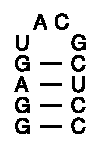
\includegraphics[width=1.5cm]{stem4.pdf} & 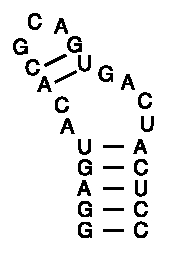
\includegraphics[width=2cm]{mk_stem.pdf} \\
	\end{tabular}
	\caption{Примеры описания структур}
\end{table}

\section{Эксперименты}

Два эксперимента: обработка баз известных 16s, обработка полноразмерных геномов.

\begin{table}[h]
	\centering
	\begin{tabular}{|c|>{\centering}p{3cm}|*{6}{C|}}
		\hline
		\multirow{2}{*}{Домен} & \multirow{2}{*}{\parbox{3cm}{\centering Стартовый нетерминал}} & \multicolumn{2}{c|}{Бактерии} & \multicolumn{2}{c|}{Эукариоты} & \multicolumn{2}{c|}{Археи} \\
		\cline{3-8}
		& & р & нр & р & нр & р & нр \\
		\hline \hline
		Центральный & h19 & 17878 & 335 & 2153 & 3165 & 306 & 13 \\
		\hline
		5'M & h3 & 10298 & 7915 & 50 & 5268 & 55 & 264\\
		\hline
	\end{tabular}
	\caption{Результаты анализа базы организмов}
\end{table}

Базы размеченных полноразмерных геномов с информацией о 16s: оценить точность, полноту и т.д. (сколько из отмеченных найдено, сколько из отмеченных не найдено, сколько найдено неотмеченных).
Проанализировать ложные срабатывания и пропущенных кандидатов.

\pagebreak

\begin{appendices}
\section{Грамматика 16S}
\label{grammar}
\verbatiminput{16S_grammar.yrd}
\end{appendices}
\end{document}